\documentclass[conference]{IEEEtran}

\usepackage{mathptmx,amssymb,amsmath}
\usepackage{stmaryrd}
\usepackage{MnSymbol}
\usepackage{float}
\usepackage{amsthm}
\usepackage{array}
\usepackage[american]{babel}
\usepackage{enumerate}
\usepackage{fancyvrb}
\usepackage{cite}
%\usepackage{url}
\usepackage{mathpartir}
\usepackage{graphicx}
\usepackage{subfig}
\usepackage{color}
\usepackage{verbatim}
\usepackage[lined,boxed,linesnumbered]{algorithm2e}

\widowpenalty=0
\clubpenalty=0
\displaywidowpenalty=0
\raggedbottom
\sloppy
\sloppypar

\topskip0pt
\parskip0pt
\partopsep0pt

\def\ind{\parindent}
\DefineVerbatimEnvironment{program}{Verbatim}
  {baselinestretch=1.0,xleftmargin=\ind,fontsize=\small,
   commandchars=\\\{\},samepage=true}
\DefineVerbatimEnvironment{programBox}{BVerbatim}
  {baselinestretch=1.0,xleftmargin=0pt,fontsize=\small,
   commandchars=\\\{\},samepage=true}

\def\denseitems{
    \itemsep1pt plus1pt minus1pt
    \parsep0pt plus0pt
    \parskip0pt\topsep0pt}

\def\exsep{1ex plus1ex}
\newcounter{exerc}
\newenvironment{exerc}%
{\refstepcounter{exerc}\vspace{\exsep}\noindent\hrulefill{}\nopagebreak\\%
 \noindent\textbf{Exercise \arabic{exerc}.}\ }
{\nopagebreak\par\vspace{-4pt}\noindent\hrulefill{}\vspace{\exsep}}

\newenvironment{exercSP}%
{\refstepcounter{exerc}\vspace{\exsep}
 \begin{samepage}\noindent\hrulefill{}\nopagebreak\\%
 \noindent\textbf{Exercise \arabic{exerc}.}\ }
{\nopagebreak\par\vspace{-4pt}\noindent\hrulefill{}
 \end{samepage}\vspace{\exsep}}


\def\defmacro#1{\expandafter\def\csname#1\endcsname}

\def\newdef#1#2{\expandafter\ifx\csname#1\endcsname\relax
    \defmacro{#1}{#2}%
    \else\message{Command "#1" already defined}\fi}

\newif\ifmore
\def\mapdef#1#2(#3){\def\args{#1:#2:#3,\end}%
    \moretrue
    \loop\expandafter\nextarg\args
         \ifmore\repeat}
\def\nextarg#1:#2:#3,#4\end{\def\next{#4}%
    \ifx\next\empty\morefalse
        \else\def\args{#1:#2:#4\end}\fi
    \newdef{#2#3}{#1{#3}}}
    
\makeatletter
\def\fixedlabel#1#2{%
  \@bsphack%
  \protected@write\@auxout{}%
         {\string\newlabel{#1}{{#2}{\thepage}}}%
  \@esphack}
\makeatother

%%%
%%% Meta notes
%%%
\newcommand{\getRef}[1]{[\textbf{** #1}: \textit{refs?}]}
\newlength{\dummylen}
\newcommand{\NOTE}[1]{\setlength{\dummylen}{\fboxrule}\setlength{\fboxrule}{2pt}%
            \vspace{1ex}\noindent\hfill%
            \fbox{\begin{minipage}{.96\columnwidth}#1\end{minipage}}%
            \setlength{\fboxrule}{\dummylen}\hfill{}\vspace{1ex}}

\definecolor{red}{RGB}{255,0,0}
\definecolor{green}{RGB}{0,255,0}
\definecolor{purple}{RGB}{255,0,255}

\DefineVerbatimEnvironment{code}{Verbatim}{fontsize=\footnotesize,fontseries=b}


%%%
%%% MATH
%%%
\def\OB#1{\ifmmode#1\else\mbox{$#1$}\fi}

% shared CC definitions
\newcommand{\OR}{\ |\ }
\newenvironment{fsyntax}{\hfill$\begin{array}{rcl@{\quad}l}}
                        {\end{array}$\hfill{\ }}
\newenvironment{syntax}{\[\begin{array}{rcl@{\quad}l}}
                       {\end{array}\]\ignorespacesafterend}
% \newenvironment{example}{\[\begin{array}{l}}
%                        {\end{array}\]\ignorespacesafterend}
\newenvironment{example}{\par\medskip\indent$\begin{array}{l}}
                       {\end{array}$\par\medskip\noindent\ignorespacesafterend}

%% overlay macros
%
\newlength{\overlaywidth}
\newlength{\overlayheight}

\newcommand{\voverlay}[3][-]{%
   \settowidth{\overlaywidth}{\mbox{\OB{#2}}}\divide\overlaywidth2%
   \hspace*{\overlaywidth}%
   \makebox[0mm]{\OB{#2}}%
   \if#1-\makebox[0mm]{\OB{#3}}\else%
         \raisebox{#1}[0mm][0mm]{\makebox[0mm]{\OB{#3}}}\fi%
   \hspace*{\overlaywidth}}

\newcommand{\vhoverlay}[3][-]{%
   \settowidth{\overlaywidth}{\mbox{\OB{#2}}}\divide\overlaywidth2%
   \settoheight{\overlayheight}{\mbox{\OB{#3}}}%
   \if#1-\else\addtolength{\overlayheight}{-#1}\fi
   \hspace*{\overlaywidth}%
   \makebox[0mm]{\OB{#2}}%
   \raisebox{-\overlayheight}[0mm][0mm]{\makebox[0mm]{\OB{#3}}}%
   \hspace*{\overlaywidth}}


%%
%% Math definitions
%%
\newtheorem{theorem}{Theorem}
\newtheorem{lemma}{Lemma}
\newtheorem{corollary}{Corollary}
\newenvironment{definition}[1][Definition]{\begin{trivlist}
\item[\hskip \labelsep {\bfseries #1}]}{\end{trivlist}}

%%% 
%%% MATH
%%%
\def\OB#1{\ifmmode#1\else\mbox{$#1$}\fi}
\newcommand{\vij}[3]{\OB{#1_{#2},\ldots,#1_{#3}}}
\newcommand{\vi}[2]{\vij{#1}{1}{#2}}
\newcommand{\vn}[2][n]{\vi{#2}{#1}}
\newcommand{\vnButi}[3][n]{\OB{#2_1,\ldots,#2_{#3-1},#2_{#3+1},\ldots,#2_{#1}}}
\newcommand{\set}[1]{\OB{\{#1\}}}
\newcommand{\vect}[1]{\OB{\langle#1\rangle}}
\newcommand{\cseq}[2][n]{\OB{^{#2:1..#1}}}
\newcommand{\iPat}[2][i]{\OB{[#1\mathop:#2]}}

% \newcommand{\xn}[1][n]{\OB{^{\bar{#1}}}}
% \newcommand{\xn}[1][n]{\OB{_{\bar{#1}}}}

\newcommand{\dom}[1]{\OB{\textit{dom}(#1)}}
\newcommand{\rng}[1]{\OB{\textit{rng}(#1)}}

\newcommand{\semL}{\OB{[\![}}
\newcommand{\semR}{\OB{]\!]}}
\newcommand{\sem}[2][{}]{\OB{\semL#2\semR_{#1}}}
\newcommand{\subst}[3]{\OB{[#1/#2]#3}}
%% multi-line definitions
\newcommand{\Begindef}{\ =\ \BegindefNES}
\newcommand{\BegindefNES}{\left\{\begin{array}{@{}l@{\quad}l}}
\newcommand{\Enddef}{\end{array}\right.}
% \newcommand{\If}{\textrm{if\ }}
\newcommand{\Otherwise}{\textrm{otherwise}}

\newcommand{\FV}[1]{\OB{\textit{FV}(#1)}}
\newcommand{\FD}[1]{\OB{\textit{FD}(#1)}}

% \newcommand{\bigstep}[3][\Delta]{\OB{#1 :- #2\Downarrow#3}}

\newcommand{\mrk}[1]{\underline{#1}}

%% 
%%  Choice calculus syntax
%%

%%% Documents and trees
% \newcommand{\prog}[1]{\texttt{#1}}
% \newcommand{\sub}[1]{\OB{{\scriptstyle\langle}#1{\scriptstyle\rangle}}}
\newcommand{\sub}[1]{\OB{\mathord\Yleft#1\mathord\Yright}}
\newcommand{\tr}[2][a]{\OB{#1\sub{#2}}}
\newcommand{\trn}[2][a]{\OB{#1\sub{\vn{#2}}}}
% \newcommand{\trPat}[4][a]{\tr[#1]{#2_{#3}|#4}}

%%% Key words & formatting/indenting
\newcommand{\CCkeyw}[1]{\textbf{\textrm{#1}}}
\newcommand{\LET}{\CCkeyw{let}}
\newcommand{\DIM}{\CCkeyw{dim}}
\newcommand{\IN}{\CCkeyw{in}}
\newcommand{\Ind}[2][{}]{\hphantom{#1}\makebox[0mm][r]{#2}\ }

%%% Choices
\newcommand{\chcL}{\langle}
\newcommand{\chcR}{\rangle}
\newcommand{\chc}[2][D]{\OB{#1\chcL#2\chcR}}
% \newcommand{\chcPP}[3][D]{\chc[#1]{\prog{#2},\prog{#3}}}

%%% Dimensions
\newcommand{\Dim}[2][D]{\OB{\DIM\ \chc[#1]{#2}}}
\newcommand{\DimIn}[3][D]{\Dim[#1]{#2}\ \IN\ #3}

%%% Let expressions
% \newcommand{\Let}[2]{\OB{\LET\ #1 = #2}\ }
% \newcommand{\Let}[3][-]{\OB{\if#1-\LET\ \else\Ind[\LET]{#1}\fi#2 = #3}}
% \newcommand{\Let}[3][\LET]{\OB{\Ind[#1]{\LET}#2 \texttt{=} #3}}
\newcommand{\Let}[3][\LET]{\OB{\Ind[#1]{\LET}#2 {\small=} #3}}
\newcommand{\LetIn}[3]{\Let{#1}{#2}\ \IN\ #3}


%%% OLD Choice notation / abbreviation
% \newcommand{\ptch}[2][L]{\OB{#2^{#1}}}
% \newcommand{\ptch}[2][L]{\OB{\overline{#2}^{#1}}}
% \newcommand{\ptch}[2][L]{\OB{#1\mathord:\ #2}}
% \newcommand{\ptch}[2][L]{\OB{#1\mathord|\ #2}}
\newcommand{\ptch}[2][L]{\OB{#1\mapsto #2}}
% \newcommand{\ptch}[2][L]{\OB{#1\to #2}}
% \newcommand{\ptch}[2][L]{\OB{#1\mathord\to #2}}
\newcommand{\ochc}[1]{\OB{\set{#1}}}
\newcommand{\chcn}[3][n]{\OB{\chc{\ptch[#2_1]{#3_1},\ldots,\ptch[#2_#1]{#3_#1}}}}
\newcommand{\ochcA}[2]{\ochc{\ptch[#1]{#2}}}
\newcommand{\ochcB}[4]{\ochc{\ptch[#1]{#2},\ptch[#3]{#4}}}
\newcommand{\ochcBi}[4]{\ochc{\ptch[\textit{#1}]{#2},\ptch[\textit{#3}]{#4}}}
\newcommand{\ochcC}[6]{\ochc{\ptch[#1]{#2},\ptch[#3]{#4},\ptch[#5]{#6}}}
\newcommand{\ochcD}[8]{\ochc{\ptch[#1]{#2},\ptch[#3]{#4},\ptch[#5]{#6},\ptch[#7]{#8}}}
%%% OLD Choice binding
\newcommand{\lbnd}[2]{\OB{#1=#2}}
\newcommand{\bnd}[2]{\OB{#1\leftarrow#2}}
\newcommand{\cbnd}[2]{\bnd{#1}{\chc{#2}}}
\newcommand{\cbind}[2]{\bnd{#1}{\chc{#2}}}
\newcommand{\bind}[3]{\OB{#1:\cbind{#2}{#3}}}
\newcommand{\bindB}[5]{\OB{#1:\cbind{#2}{#3};\cbind{#4}{#5}}}
\newcommand{\bindk}[3]{\OB{#1:\cbind{#2_1}{#3_1};\ldots;\cbind{#2_k}{#3_k}}}
\newcommand{\bindkC}[3]{\OB{#1:\bnd{#2_1}{#3_1};\ldots;\bnd{#2_k}{#3_k}}}
\newcommand{\noDbindkC}[2]{\OB{\bnd{#1_1}{#2_1};\ldots;\bnd{#1_k}{#2_k}}}
\newcommand{\noCode}{\OB{\bullet}}
\newcommand{\tagsName}{\textit{tags}}
\newcommand{\tags}[1]{\OB{\tagsName(#1)}}
\newcommand{\ctags}[1]{\OB{\textit{ctags}(#1)}}
\newcommand{\ddom}[1]{\OB{\textit{dom}^*(#1)}}

%% formatting choice names/ids
% \newcommand{\choice}[1]{\OB{{\cal #1}}}

%% names for change objects
% \newcommand{\chObj}{\OB{\omega}}
% \newcommand{\chObjB}{\OB{\omega'}}
% \newcommand{\chObj}{\OB{\bar{O}}}
% \newcommand{\chObjB}{\OB{\bar{O'}}}
% \newcommand{\vo}{\OB{\bar{O}}}
% \newcommand{\vo}{\OB{V}}
% \newcommand{\voB}{\OB{V'}}


%%
%% Static analysis
%%
\newcommand{\wdim}[2][\Delta]{\OB{#1\vdash#2}}

%%% Context notation
% \newcommand{\ctx}[1]{\OB{^{\sswarrow}C[#1]}}
%\newcommand{\ctx}[1]{\OB{\hat{C}[#1]}}
\newcommand{\ctx}[2][C]{\OB{#1[#2]}}


%%% Tag selection
\newcommand{\sel}[2][D.t]{\OB{#2\mathop\shortuparrow#1}}
% \newcommand{\tsel}[3][\Delta]{\OB{#2|_{#1}^{#3}}}
\newcommand{\tsel}[2][s]{\OB{\lfloor#2\rfloor_{#1}}}
% \newcommand{\tsel}[3][\Delta]{\OB{\sigma(#1,#2,#3)}}
% \newcommand{\tseltd}[2][\Delta]{\tsel[#1]{#2}{d.t}}
% \newcommand{\tselq}[2][\Delta]{\tsel[#1]{#2}{q}}

\newcommand{\dimSym}{\OB{\delta}}
\newcommand{\dims}[1]{\dimSym(#1)}
\newcommand{\dimProd}{\OB{\otimes}}
\newcommand{\dimSum}{\OB{\oplus}}
\newcommand{\dimUnit}{\textbf{1}}

\newcommand{\expSym}{\OB{\mu}}
\newcommand{\expEnv}{\OB{\rho}}
\newcommand{\expand}[2][\expEnv]{\expSym_{#1}(#2)}


\newcommand{\chcdep}[2]{\OB{#1\leftarrow#2}}

%% name of positional relationship
% \newcommand{\prel}{\OB{\Delta}}
% 
% \newcommand{\mkchc}[3][p]{\OB{#2[#1]\mathord{:}#3}}
% \newcommand{\addchc}[3][p]{\OB{#2[#1]\mathord{:}\mathord\cup#3}}
% \newcommand{\chcex}[2][p]{\OB{#2_{#1}}}

%% 
%%  Choice calculus semantics
%%

\newcommand{\tselB}[3]{\tsel[#3]{\tsel[#2]{#1}}}
\newcommand{\lft}[1]{\OB{\mathord\uparrow#1}}
\newcommand{\plain}[1]{\OB{\underline{#1}}}
\newcommand{\allsel}[2]{\OB{#1\mathord\Downarrow#2}}
% \newcommand{\lsel}[2][t_1,\ldots,t_n]{\OB{#2.\set{#1}}}

%%% Dimensions
\newcommand{\choicesSym}[1][{}]{\OB{\Gamma^{#1}}}
\newcommand{\choices}[2][{}]{\OB{\choicesSym[#1](#2)}}
\newcommand{\dimm}[1]{\dimSym(#1)}

%%% Variations
\newcommand{\variSym}{\OB{V}}
\newcommand{\vari}[1]{\OB{\variSym(#1)}}


%% 
%%  Design theory
%%
\newcommand{\equivSym}{\OB{\sim}}

\newcommand{\equalt}[3][C]{\OB{#2\equivSym_{#1}#3}}
\newcommand{\equtag}[3][C]{\OB{#2\equivSym_{#1}#3}}

% \newcommand{\dropName}{\textit{rem}}
% \newcommand{\drop}[4][C]{\OB{\dropName\textit{#2}_{#1}^{#3}(#4)}}
% \newcommand{\dropA}[3][C]{\drop{A}{#2}{#3}}
% \newcommand{\dropT}[3][C]{\drop{T}{#2}{#3}}
% \newcommand{\dropA}[3][C]{\OB{\alpha_{#1}^{#2}(#3)}}
% \newcommand{\dropA}[3][C]{\OB{\alpha_{#2}^{#1}(#3)}}


\newcommand{\dropi}[4][C]{\OB{\bar{#2}_{#1/#3}(#4)}}
\newcommand{\drop}[3][C]{\OB{\bar{#2}_{#1}(#3)}}

\newcommand{\dropA}[3][C]{\dropi[#1]{\alpha}{#2}{#3}}
\newcommand{\dropT}[3][C]{\dropi[#1]{\tau}{#2}{#3}}
\newcommand{\dropC}[2][C]{\drop[#1]{\gamma}{#2}}
\newcommand{\dropD}[2][C]{\drop[#1]{\delta}{#2}}



\newcommand{\vequiv}[2]{\OB{#1\sim#2}}
\newcommand{\tequiv}[4][e]{\OB{#3\equivSym^{#1}_{#2}#4}}
\newcommand{\tsubst}[4][D]{\OB{[#1:#2/#3]#4}}




%%% Properties of dimensions
% \newcommand{\indep}[2]{\OB{#1\rightleftarrows#2}}
% \newcommand{\depnd}[2]{\OB{#1\Leftarrow#2}}
\newcommand{\indep}[2]{\OB{#1\mathop\|#2}}
\newcommand{\related}[2]{\OB{#1\mathop\sim#2}}
\newcommand{\relclSym}{\OB{\vhoverlay[1.6ex]{\sim}{\scriptstyle *}}}
% \newcommand{\relclSym}{\OB{\overset{*}{\sim}}}
\newcommand{\relcl}[2]{\OB{#1\,\relclSym\,#2}}
\newcommand{\depnd}[2]{\OB{#1\rightarrow#2}}
\newcommand{\synch}[2]{\OB{#1\leftrightarrow#2}}
\newcommand{\ovlap}[2]{\OB{#1\leftrightharpoons#2}}


%%% Operations on versioned objects
\newcommand{\factorSym}{\OB{\varphi}}
\newcommand{\factor}[1]{\OB{\factorSym(#1)}}
\newcommand{\distrSym}{\OB{\delta}}
\newcommand{\distr}[1]{\OB{\distrSym(#1)}}


%%% Java example
% \newcommand{\etc}{\OB{\cdots}}
% \newcommand{\etc}{}
\newcommand{\tok}[1]{\texttt{\small #1}}
\newcommand{\toktr}[2]{\tr[\tok{#1}]{#2}}
\newcommand{\Nesting}[2]{\begin{array}[b]{@{}l@{}}%
     \tok{#1}\langle\\ \indnt#2\end{array}}
\newcommand{\End}{\rangle}
\newcommand{\indnt}{\hspace*{1em}}

\newcommand{\showEx}[1]{\medskip\noindent\centerline{#1}\medskip\noindent}

\newcommand{\class}[1]{\toktr{class}{#1}}
% \newcommand{\classNest}[1]{\Nesting{class}{#1}}
\newcommand{\List}{\tok{List}}
\newcommand{\Listg}{\tok{List<Job>}}
\newcommand{\voidName}{void}
\newcommand{\void}[1]{\toktr{\voidName}{#1}}
\newcommand{\intt}{\tok{int}}
\newcommand{\Iter}{\tok{Iter}}
\newcommand{\while}[1]{\toktr{while}{#1}}
\newcommand{\forr}[1]{\toktr{for}{#1}}
\newcommand{\Job}{\tok{Job}}
\newcommand{\run}{\tok{j.run}}
\newcommand{\ifff}{\tok{if}}
\newcommand{\nocode}{\OB{\bullet}}

% alternative content-based naming
\renewcommand{\voidName}{runJob}
\renewcommand{\intt}{\tok{trialCount}}
\renewcommand{\ifff}{\tok{break}}

\newcommand{\prel}{\OB{{\cal R}}}

% class, List/List<Job>, runJobs, trialCount, Iter, for/while, Job, j.run, break





% General language structure
%
\newcommand{\prog}[1]{{\small\texttt{#1}}}
\newcommand{\bs}{\texttt{\symbol{92}}}

\newcommand{\lblFmt}[1]{\textrm{\textit{#1}}}
\newcommand{\chcPP}[3][D]{\chc[#1]{\prog{#2},\prog{#3}}}
\newcommand{\chcPPP}[4][D]{\chc[#1]{\prog{#2},\prog{#3},\prog{#4}}}

% dimensions and tags
\newcommand{\dimA}[2][a_1,a_2]{\DimIn[A]{#1}{#2}}
\newcommand{\chcA}[1]{\chc[A]{#1}}
\newcommand{\dcA}[2][a_1,a_2]{\dimA[#1]{\chcA{#2}}}

\newcommand{\dimB}[2][b_1,b_2]{\DimIn[B]{#1}{#2}}
\newcommand{\chcB}[1]{\chc[B]{#1}}
\newcommand{\dcB}[2][b_1,b_2]{\dimB[#1]{\chcB{#2}}}

%%
%% Duc's def
%%
\newcommand{\figscale}{0.6}
\newcommand{\varsheet}{VarSheet}
\newcommand{\EUSES}{EUSES}
\newcommand{\gds}{goal-directed selection}

\newcommand{\da}{\OB{r}}
\newcommand{\spos}{\OB{p}}
\newcommand{\f}{\OB{f}}
\newcommand{\add}{\OB{a}}
\newcommand{\gid}{\OB{id}}
\newcommand{\tg}{\OB{t}}
\newcommand{\tgs}{\OB{2^t}}
\newcommand{\F}{\OB{F}}
\newcommand{\vsheet}{\OB{s}}
\newcommand{\VSheet}{\OB{S}}
\newcommand{\V}[1]{\OB{V~#1}}
\newcommand{\TCons}{\OB{\prog{T}}}
\newcommand{\mapname}[1]{\textit{#1}}
\newcommand{\dset}[1]{\{#1\}}
\newcommand{\gcell}[1]{\##1}
\newcommand{\ltText}{\OB{<_{r}}}
\newcommand{\eqText}{\OB{\equiv_{r}}}
\newcommand{\ltRel}[2]{#1 \ltText #2}
\newcommand{\eqRel}[2]{#1 \eqText #2}

\newcommand{\htdim}{Housing\&Transportation}
\newcommand{\lpdim}{Loan Payment}

\pagestyle{plain}
\date{}

\begin{document}

\title{A Model for Representing Variational Spreadsheets
\thanks{This work is partially
supported by the Air Force Office of Scientific
Research under the grant FA9550-09-1-0229 and by the
National Science Foundation under the grant CCF-0917092.
}}

\author{
\IEEEauthorblockN{Martin Erwig}
\IEEEauthorblockA{Oregon State University\\
                  erwig@eecs.oregonstate.edu}
\and
\IEEEauthorblockN{Duc Le}
\IEEEauthorblockA{Oregon State University\\
                  ledu@eecs.oregonstate.edu}
\and
\IEEEauthorblockN{Eric Walkingshaw}
\IEEEauthorblockA{Oregon State University\\
                  walkiner@eecs.oregonstate.edu}
}

\maketitle

\begin{abstract}
TBD
\end{abstract}

\section{Introduction}
\label{sec:intro}

\NOTE{New motivation needed}

We first give a motivating example for \varsheet. Figure~\ref{fig:before} shows a conventional spending estimate of
a college student. Suppose the student is not happy with it,
they would adjust the costs of some categories based on available options. After some adjustments, the student ends up with the spreadsheet in Figure~\ref{fig:after}, for which they pay \$50 less.
In the updated spreadsheet, the housing cost is \$50 less since the rented house is further from campus, but that would increase
the cost of transportation. The student also decides to pay \$100 less on their loan.
Considering both versions, the student would probably go after the latter one, and by doing this, they lose
the chance to reduce another \$50. Had the student chosen the original housing option and kept Loan payment to be \$500, the monthly
cost would have been \$1450.

Figure~\ref{fig:selection} shows a possible user interface of \varsheet~that could support the student in their decision making process.
There are three variation points in the spreadsheet. The \mapname{\htdim} categories are related and thus grouped
into a red box with a dashed line separating the two available options. 
In \varsheet, \mapname{\htdim} is called a \emph{dimension}---a choice users have to make. A dimension contains a set of options, each being called a \emph{tag}.
\mapname{\htdim}'s tags are \mapname{Close} and \mapname{Far}.
The \mapname{\lpdim} dimension represents a different variation point with two tags \mapname{500} and \mapname{600}
 and thus is colored differently (green). 
The last variation point, the \mapname{Total} category, does not contain variational formulas by itself. The formula being
used is \prog{SUM(B2:B6)} and is non-variational, yet the cell inherits the variational structures of its referred cells and
hence contains four available options. This cell is therefore colored purple to indicate that it contains \emph{induced variation}. Showing all the four alternatives of 
\mapname{Total} gives the student an overview of all the different options they
have. Moreover, if the student selects the \$1450 alternative, \varsheet~will automatically make
decisions for \mapname{\htdim} and \mapname{\lpdim}, and displays those decisions and the resulting spreadsheet to them.
We call this feature \emph{\gds}, the process of selecting spreadsheet variants based on certain goals.

\begin{figure}
\centering
    \subfloat[Before] {
        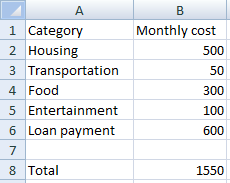
\includegraphics[scale=\figscale]{img/before}
        \label{fig:before}
    }\hspace{2em}
    \subfloat[After] {
        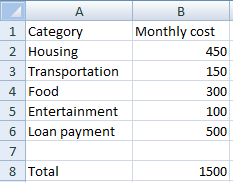
\includegraphics[scale=\figscale]{img/after}
        \label{fig:after}
    }\hspace{2em}
    \subfloat[A Possible User Interface] {
        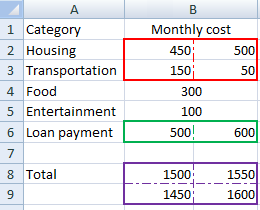
\includegraphics[scale=\figscale]{img/selection}
        \label{fig:selection}
    }
\caption{A Monthly Spending Spreadsheet}
\label{fig:mspending}
\end{figure}



The study of variational spreadsheets brings up several insights to current research on software variation.
While traditional variation mechanisms focus on either the syntax or semantics domain, spreadsheets' immediate semantics computation expands the application of variational constructs to both domains, enabling the realization of \gds. 
In the example above, Loan payment varies syntactically while Total varies semanticallly, and one could even define cells that vary on both domains.

Existing variational contructs mainly work on linear or tree structures, which localizes their scope of impact. 
Spreadsheets have a special two dimensional structure that makes localization hard to achieve.
For instance, in Figure~\ref{fig:before}, one could replace row 4 by the spreadsheet in Figure~\ref{fig:food} and
expects this variation introduction to be local. This action unfortunately has a global impact on the spreadsheet's structure and the addresses/values of several unrelated cells.
The Monthly Cost column has to be shifted to column C, while the Total column has to be shifted one row down. 
In our variational spreadsheet model, we provide mechanisms to localize the effect of structural changes.

\begin{figure}
\centering
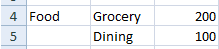
\includegraphics[scale=\figscale]{img/food}
\caption{A Different Way to Represent the Food Category}
\label{fig:food}
\end{figure}

Lastly, by letting users actively define variation in spreadsheets, we remove the need for using spreadsheet diffing algorithm,
which can be imperfect and misleading at times.

% In following sections of the paper, we first discuss the background and related work in section~\ref{sec:background}. Then we
% begin describing the syntax of \varsheet~in section \ref{sec:syntax}, which is followed by section \ref{sec:semantics} about the language's semantics.
% Section \ref{sec:langprops} discusses several axiomatic rules that could be used to transformed,
% while section \ref{sec:eval} provides an evaluation of our language on the \EUSES~corpus \cite{Ii05theeuses}. Section \ref{sec:concl} concludes the paper.

\section{Background and Related Work}
\label{sec:background}

\NOTE{To be rewritten}

\NOTE{Talk about the prototype of the VLHCC 2011 paper}

Existing empirical research demonstrates the need for an effective approach to deal with spreadsheet variation.
Spreadsheet reusing is common, but users often have to choose from various options [citation needed].
Once a spreadsheet is chosen and several modifications have been made to it,
if users recognize that it was not the right one to begin with, they will have to start all over again on a
different one. This could happen for many times until users are happy with their choice. To mitigate this problem, \varsheet~
gives users the ability to modify multiple versions/spreadsheets at the same time on a single representation and
select a desired version later.
Another reason for spreadsheet variation is due to spreadsheet errors and debugging.
Spreadsheets contain errors \cite{Panko98whatwe}\cite{Powell2008128}, many of which are introduced in the process of
reusing and modifying existing spreadsheets. When debugging, users often need to show the
differences between multiple versions, so a framework for systematically managing changes is needed.

In the area of spreadsheet change support, existing tools can be classified into two big categories: change tracking tools and spreadsheet diffing tools.
One representative example of a change tracking tool is Microsoft Excel's change tracking feature, which provides users the ability to track spreadsheet edits
such as inserting rows, updating equations, etc. This tool is useful and effective in helping users
understand versioning information of spreadsheets but is not
without limitation. The entire variational spreadsheet is represented using only the time dimension. It is not possible
to group changes into categories or groups such that they can be undone or applied again. Another problem arises when two or more users copy and modify
the same original spreadsheet. When trying to merge the modified copies, it is unclear which change includes or excludes other changes.
For \varsheet, grouping changes could simply be resolved by changing dimension/choice names, which will be defined in the next sections.
Research and commercial tools for diffing spreadsheets are prevalent, including CC DiffEngineX \cite{DiffEngineX} and Synkronizer \cite{Synkronizer}.
These tools are effective in comparing spreadsheets and producing accurate results. However, they do not reveal the original purposes
of users' changes and do not provide a way to document those.

On a broader topic, there has been extensive research on the topic of representing and managing software variation. The two big pillars of this topic
is the compositional approach \cite{KA08}, which modularizes software product line features \cite{CN01} into individual folders and
describes variability at a higher level using feature models \cite{Bat05}, and the annotated approach \cite{KA08}, where variability is encoded
and represented inside source code. Since there are advantages and disadvantages for each approach, Erwig and Walkingshaw~\cite{EW11tosem}
designed the Choice Calculus to shorten the gap between them and to take advantage of the approaches' benefits. The Choice Calculus's design
is based on the idea that software variation should be done at both source code and higher
levels with not-too-restrictive and not-too-relaxed constraints, making it highly
applicable for tree-like structures. \varsheet~expands Choice Calculus's ideas of dimensions
and choices to the spatial, two dimensional structure of spreadsheets.

% \varsheet~reuses several Choice Calculus constructs and semantics in the domain of spreadsheet computing.
% Hence, many of the existing results of the Choice Calculus will still be applicable in the context of the \varsheet~language.

%\section{Syntax}
%\label{sec:syntax}

\section{\varsheet's Design}
\label{sec:design}

\varsheet's design follows the annotative approach and encodes variation at the most fine-grained
level---the cell level. Every single cell is annotated with a description about which variant it belongs to.
A variational spreadsheet represents a universe of annotated cells from
which one could pick subset to form a variant.
By convention, users only see individual variants, yet they can go into
\emph{variational exploration mode} to explore all alternatives of a cell or a set of cells (as in Figure~\ref{fig:selection}).
Each cell is associated with a distinct global identity.
Formally, a variational spreadsheet is a partial function from the set of global identities to
sets of tags, \emph{relative spatial positions}, and formulas.

\begin{equation}
\label{eq:vsheet}
\vsheet \in \VSheet = \gid \rightarrow (2^{\tg}, \spos, \f)
\end{equation}

In the above definition, \vsheet~stands for variational spreadsheets, \gid~ranges over global 
identities\footnote{We assume the set of global identities is an
infinite set from which fresh, unused identities can be drawn. In this paper, we use natural numbers to represent global identities.}, 
\tg~stands for tags, $2^{\tg}$ is the power set of all tags, \spos~represents relative partial positions (more on this later), and \f~represents formulas.
Each cell can then be encoded as a tuple (\gid, \tgs, \spos, \f).

\subsection{Dimensions and Tags}
\label{sec:dimtag}

\begin{definition}
A \emph{dimension} consists of a set of options, each being called a \emph{tag}.
\end{definition}

\noindent
We distinguish tags having identical names by qualifying them with dimension names (e.g. \mapname{\htdim.Close}).
Dimensions and tags form the basis for how variational spreadsheets vary.
Every variational spreadsheet can constitute several independent dimensions, each of which represents an independent choice users have to make.
Every cell contains tags to decide which variant the cell belongs to.

\begin{definition}
A \emph{decision} is a set of tags from different dimensions.
A \emph{complete decision} is a decision with tags from all dimensions in a variational spreadsheet.
\end{definition}

A decision can be an empty set ($\emptyset$), a set of a single tag (\dset{\mapname{\htdim.Close}}), or a set of multiple tags (\dset{\mapname{\htdim.Close, \lpdim.500}}).
Decisions provide means for selecting individual variants from variational spreadsheets.
Given the decision \dset{\mapname{\htdim.Close, \lpdim.600}}, the variant in Figure~\ref{fig:before}~is selected. Given the decision \dset{\mapname{\htdim.Far, \lpdim.500}}, the variant in Figure~\ref{fig:after}~is selected.

\begin{figure*}
\centering
\subfloat[Variant 1]{
    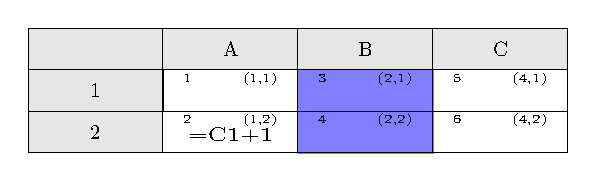
\includegraphics[scale=\figscale]{tikz/v1}
    \label{fig:v1}
}
\subfloat[Variant 2]{
    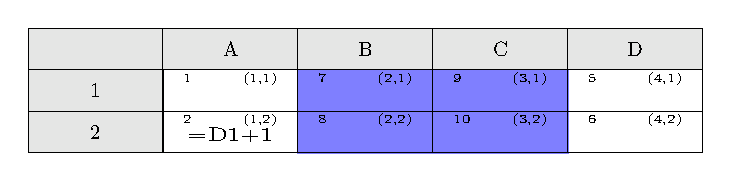
\includegraphics[scale=\figscale]{tikz/v2}
    \label{fig:v2}
}
\caption{Two variants of a variational spreadsheet}
\label{fig:idedsheet}
\end{figure*}

In Figure~\ref{fig:idedsheet} we provide two variants of a variational spreadsheet containing a single dimension \mapname{D} with two tags \mapname{D.1} and \mapname{D.2}.
As the consequence, there are two decisions, \dset{\mapname{D.1}} and \dset{\mapname{D.2}},
the former associating with variant 1 while the latter with variant 2.
On the top-left corner of each cell is its global identity. We leave
the contents of several cells blank as they are not important for our discussion.
Two different types of cells exist in Figure~\ref{fig:idedsheet}, \emph{non-variational} and \emph{variational} cells.
Non-variational cells are cells that appear in all variants whereas variational cells do not. Cells with ID 1, 2, 5, 6 are non-variational (from now on we will use the convention: cell \gcell{1}, \gcell{2}, \gcell{5}, \gcell{6}), and all other cells are variational ones. 
Non-variational cells' tags are empty sets while variational cells' tags are non-empty.
We provide the cells' tags below.

\[
\begin{array}{l@{\ : \ }l}
    \gcell{1}, \gcell{2}, \gcell{5}, \gcell{6} & \emptyset \\
    \gcell{3}, \gcell{4} & \dset{\mapname{D.1}} \\
    \gcell{7}, \gcell{8}, \gcell{9}, \gcell{10} & \dset{\mapname{D.2}} \\
\end{array}
\]

% \NOTE{Talk about relative position + pretty printing algorithm.
% Then talk about formula, global referencing.}
\subsection{Relative Spatial Positions and Formulas}
\label{sec:relpos_form}

Figure~\ref{fig:idedsheet} gives an example of \emph{structural variation}, where
a 2x1 sub-spreadsheet in variant 1 was replaced by a 2x2 sub-spreadsheet in variant 2.
In each variant, there is a reference from the cell \gcell{2} to the cell \gcell{5}.
The formula of cell \gcell{2} changes when we switch from one variant to the other (from \prog{=C1+1} to \prog{=D1+1} and vice versa), which surprisingly
implies that cell \gcell{2} is influenced by the decision in dimension \mapname{D}, which should not be the case.
This results from the fact that structural changes in spreadsheets
have global impact, and we need a mechanism to reduce the scope of impact to the minimal.

Instead of using conventional spreadsheets' absolute/relative address referencing schemes, we employ
in our model a \emph{global identity referencing scheme} in which the formula of \gcell{2} is \prog{=\gcell{5}+1}.
When the first variant of the spreadsheet is shown, \gcell{5}'s address is mapped to \prog{C1}, and
when the second variant is selected, \gcell{5}'s address is mapped to \prog{D1}, so the formula of \gcell{2} is displayed according to the selected variant.
The definition for spreadsheet formulas is thus defined as

\[
\begin{array}{lcl@{\qquad}l}
\f \in \F & ::= & v  & \textit{values} \\
         & \OR & \gid & \textit{identity references} \\
         & \OR & \OB{\omega} (\f, \ldots, \f) & \textit{functions}\\
\end{array}
\]

\newcommand{\natset}{\OB{\mathbb{N}}}
\newcommand{\strset}{\OB{\mathbb{S}}}
\noindent
Note that we store identity references but show normal address references to users.
As cell definitions do not encode address information, the burden now
lies on how to map cell identities to addresses. We solve this problem by defining a pretty 
printing algorithm for variants. 
%
The process of selecting a variant is 
similar to picking a subset of cells from the universe of cells. 
Each cell in the subset carries information about its \emph{relative spatial position},
which is used to aid the pretty printing algorithm in deciding cell addresses.
Relative spatial positions are pairs of natural numbers, \spos~= (\natset, \natset), the first element representing relative
vertial positions and the second representing relative horizontal positions.
In Figure~\ref{fig:idedsheet}, spatial positions are shown on the top-right corner
of each cell. Normal cell addresses are pairs of strings and natural numbers, \add~= \OB{(\strset, \natset)}. 

The pretty printing algorithm (presented in Algorithm~\ref{alg:prettyprint}) takes a set of cells as input and attaches an addresses to each cell (e.g. \gcell{1} will have the address \prog{A1}).
This algorithm assumes the left-most and top-most cell's address
is \prog{A1}.

\begin{algorithm}
    \SetKwData{posset}{P}
    \SetKwData{vposset}{VP}
    \SetKwData{hposset}{HP}
    \SetKwData{cellset}{C}
    \SetKwData{cell}{c}
    \SetKwData{cadd}{cadd}
    \SetKwData{radd}{radd}
    \SetKwData{ret}{ret}
    \SetKwData{v}{v}
    \SetKwData{h}{h}
    \SetKwFunction{ptag}{tag}
    \SetKwFunction{tagLookUp}{tagLookUp}
    \SetKwInOut{Input}{input}
    \SetKwInOut{Output}{output}
    \Input{A set \cellset of cells, each being encoded with (\gid, \tgs, \spos, \f)}
    \Output{A mapping between cells and addresses}
    \BlankLine
        Extract the set of positions \posset from \cellset\;
        The set of vertical positions \vposset = $\{x\ |\ (x, y) \leftarrow \posset \}$ \;
        The set of horizontal positions \hposset = $\{y\ |\ (x, y) \leftarrow \posset \}$ \;
        Sort elements in \vposset and \hposset in ascending order \;
        Tag the first element in \vposset with ``\prog{A}'', the second with ``\prog{B}'' and so on\;
        Tag the first element in \hposset with \prog{1}, the second with \prog{2} and so on\;
        \ret $\leftarrow \emptyset$\;
        \For{\cell $\in$ \cellset} {
            \v $\leftarrow$ \cell's vertical position\;
            \h $\leftarrow$ \cell's horizontal position\;
            \cell's column address \cadd $\leftarrow$ \tagLookUp{\vposset, \v}\; 
            \cell's row address \radd $\leftarrow$ \tagLookUp{\hposset, \h}\;
            \ret $\leftarrow$ \ret $\cup$ \{(\cell, (\cadd, \radd))\}\;
        }
        \Return{\ret}\;
    \caption{Pretty Printing Spreadsheet Variants}
    \label{alg:prettyprint}
\end{algorithm}


\section{Semantics}
\label{sec:semantics}
\newcommand{\semP}{\sem[P]}

The pretty printing algorithm works on individual variants, which are selected by picking a subset of cells from the cell universe.
A natural question is how do we know which cell to pick. To answer this question,
in this section we describe \emph{variation semantics}, a mapping between complete decisions and spreadsheet variants.\footnote{Note that
we ignore the discussion about the semantics of individual variants since
they are basically the semantics of plain spreadsheets.}

The steps involved in computing variation semantics are: (1) collecting
the set of dimensions, (2) generating all complete decisions,
and (3) performing \emph{tag selection} on those decisions to produce variants.

\subsection{Dimensions and Complete Decisions}
\newcommand{\dimColText}{\textit{dims}}
\newcommand{\dimCol}[1]{\OB{\dimColText(#1)}}
\newcommand{\tagsText}{\textit{tags}}
\newcommand{\tagsCell}[1]{\OB{\tagsText(#1)}}
\newcommand{\decisionsText}{\textit{decisions}}
\newcommand{\decisions}[1]{\OB{\decisionsText(#1)}}
\newcommand{\examplesheet}{\OB{sh}}

We define the \dimColText~operation for collecting
all dimensions in a variational spreadsheet.
For the spreadsheet in Figure~\ref{fig:mspending}, \dimColText~returns \{\mapname{\htdim}, \mapname{\lpdim}\}. 
The set of complete decisions of a variational spreadsheet \vsheet~is defined as
\begin{align*}
\decisions{\vsheet} = \{D_1.t_1, \ldots, D_k.t_k\ |\ \{D_1,\ldots,D_k\} = \dimCol{\vsheet},t_i \leftarrow D_i\}
\end{align*}


\subsection{Tag Selection}

The tag selection procedure $\tsel[ts]{\vsheet}$~takes a complete decision \OB{ts} and goes through
a variational spreadsheet \vsheet~to filter out all cells whose tags are subsets of \OB{ts} into a variant.

% The two tag sequences $\OB{ts_1}$ and $\OB{ts_2}$ are compatible
% when either $ts_1 \subseteq ts_2$ or $ts_2 \subseteq ts_1$.
\[
\tsel[ts]{\vsheet} = \{c\ |\ c \leftarrow \vsheet, \tagsCell{c} \subseteq ts\}
\]
\noindent
Notice the \tagsText~operation, which selects a variational cell's tags .

Variation semantics is then defined as
\[
\begin{array}{r@{\ =\ }l}
    \vari{\vsheet} & \{(ts, \tsel[ts]{\vsheet})\ |\ ts \leftarrow \decisions{\vsheet}\} \\
\end{array}
\]

For the spreadsheet in Figure~\ref{fig:idedsheet}, the decisions are \dset{\mapname{D.1}} and \dset{\mapname{D.2}}.
Given each cell's tags, \dset{\mapname{D.1}} is mapped to
the set of cells \{\gcell{1}, \gcell{2}, \gcell{3}, \gcell{4}, \gcell{5}, \gcell{6}\}, and \dset{\mapname{D.2}} is mapped to
the set of cells \{\gcell{1}, \gcell{2}, \gcell{5}, \gcell{6}, \gcell{7}, \gcell{8}, \gcell{9}, \gcell{10}\}.
These two sets then become inputs for the pretty printer to
generate cell addresses.

\section{Concrete Syntax}
\label{sec:concsyntax}

The concrete syntax has two different modes: the \emph{variation exploration} mode and the default \emph{individual variant} mode.
In the variation exploration mode, users can expand several variation points to show all the available alternatives as
in Figure~\ref{fig:selection}. Users can also select a certain alternative of a variation point and corresponding decisions 
will be made automatically. The individual variant mode displays individual variants to users. 
To see a variant, users make decisions using the dimension panel as in
Figure~\ref{fig:dimension_panel}, which visualizes the relationship between dimensions and tags.
All tags of a dimension are grouped into a radiobutton group.
Users make decision for that dimension by selecting one of the radiobuttons.
The idea of dimension panel is reused from our previous work on variational representation of source code \cite{le2011}.
This work confirmed that showing individual variants and separating the configuration structures into a dimension panel improved program comprehension.

Each dimension is mapped to a distinct color and all cells relating to that dimension is annotated with
the same color.
This matching is only applicable when a cell's tags has only one dimension.
When a cell is associated with two or more dimensions, we could apply different visual cues to represent the relationship.
One approach could be creating a color palette at one of the cell's corner for storing the colors of all associated dimensions. Another approach is using a special color for the cell to indicate its dependence on multiple dimensions
and then when the cell is highlighted, all related dimensions are also highlighted in the dimension panel.

\begin{figure}
\centering
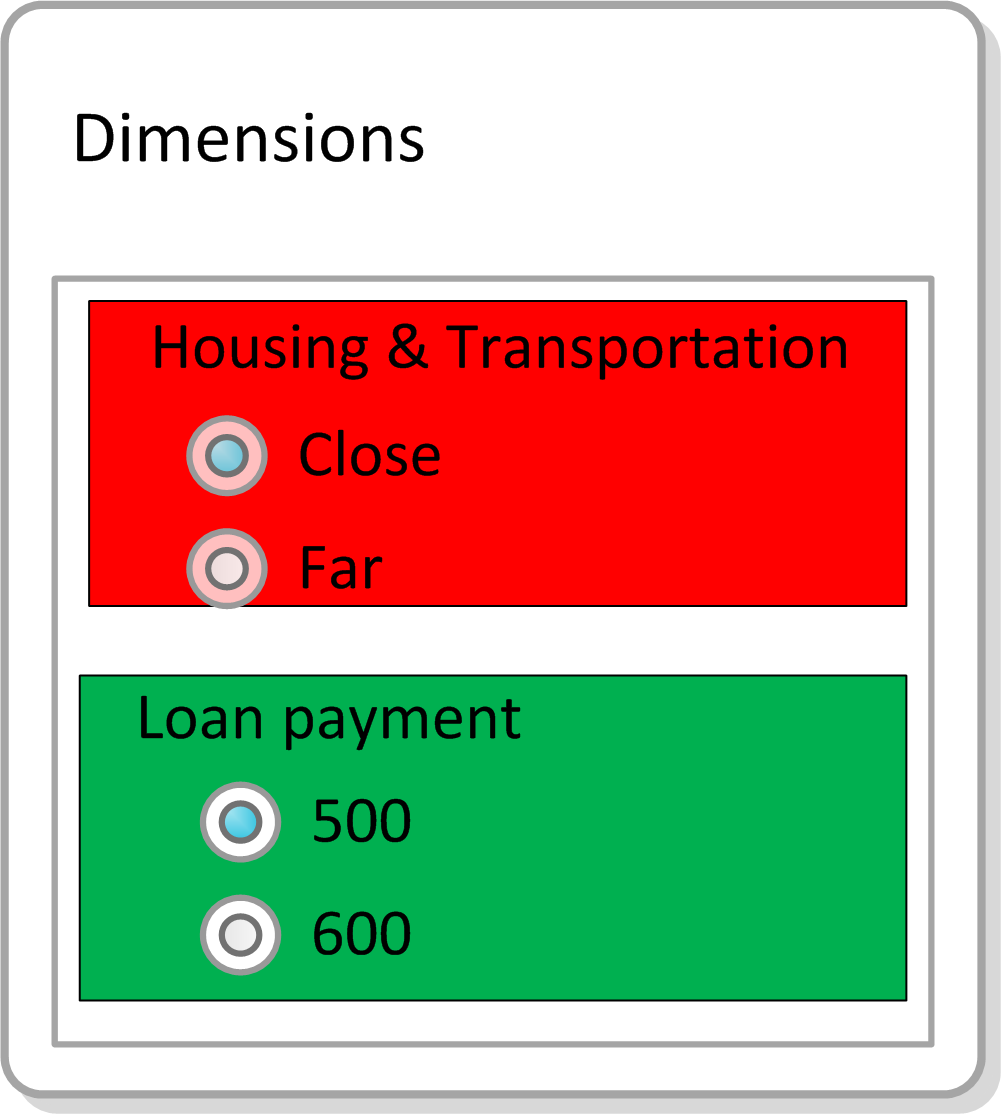
\includegraphics[scale=\figscale]{img/dimension_panel}
\caption{Dimension Panel}
\label{fig:dimension_panel}
\end{figure}

Producing the concrete presentation of spreadsheet variants requires taking the output of the
pretty printer and positioning cells at appropriate addresses.
We require that each variant has a rectangular shape, which results in cases where one
has to add \emph{filler cells} to fill up empty spaces.
Table~\ref{tbl:fourvar} gives an example where filler cells are needed. 
There are four variants of a variational spreadsheet with two dimensions $D = \{D_1, D_2\}$ and $D' = \{D'_1, D'_2\}$.
The column and row headers represent the corresponding decision of each variant.
For instance, the decision \dset{$D_1, D'_2$} corresponds to the lower left variant.
Each cell's tags are listed below.
\[
\begin{array}{l@{\ : \ }l}
    \gcell{1} & \dset{D_1} \\
    \gcell{2} & \dset{{D'_1}} \\
    \gcell{3}, \gcell{4} & \dset{D_1} \\
    \gcell{5}, \gcell{6} & \dset{{D'_2}} \\
\end{array}
\]
Cell \gcell{7} and \gcell{8} are filler cells, that is, they are not represented or stored in our model, yet
they are needed to ensure variants' rectangular shapes. Cell \gcell{7} is added whenever $D'_2$ is chosen.
For example, our semantics function maps the decision \dset{$D_1, D'_2$} to the set of three cells \{\gcell{1}, \gcell{5}, \gcell{6}\}.
The pretty printer then generates the corresponding addresses for each of these cells.
\[
\begin{array}{l@{\ : \ }l}
    \gcell{1} & \prog{A1} \\
    \gcell{5} & \prog{B1} \\
    \gcell{6} & \prog{B2} \\
\end{array}
\]
Since address \prog{A2} is not occupied by any cell, it becomes a ``black hole'' and is filled with cell \gcell{7}.
While cell \gcell{7} is added when a singular choice $D'_2$ is chosen, \gcell{8} requires two choices $D_2$ and $D'_2$ 
to be added to corresponding variants.

\NOTE{TODO: Get rid of relative postions from \gcell{7} and \gcell{8} in Table~\ref{tbl:fourvar}}

\begin{table*}
\centering
  \begin{tabular}{|>{\centering\arraybackslash}m{2em}|>{\centering\arraybackslash}m{18em} >{\centering\arraybackslash}m{25em}|}
    \hline
    & $D_1$ & $D_2$ \\ \hline
    $D'_1$ & 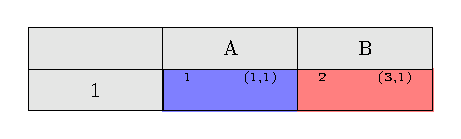
\includegraphics[scale=\figscale]{tikz/2dims1} 
      & 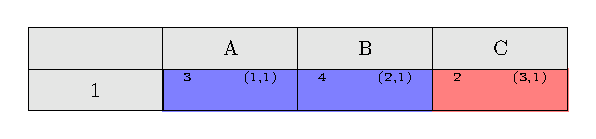
\includegraphics[scale=\figscale]{tikz/2dims2} \\
      $D'_2$ & 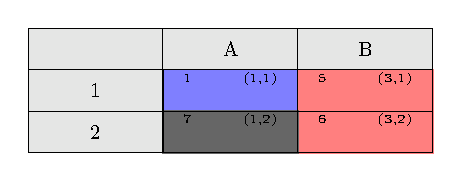
\includegraphics[scale=\figscale]{tikz/2dims3}
      & 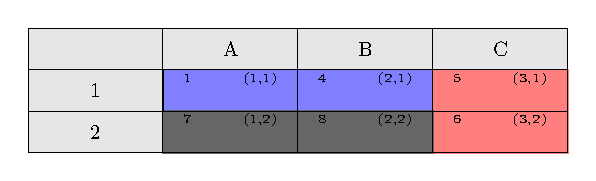
\includegraphics[scale=\figscale]{tikz/2dims4} \\ \hline
  \end{tabular}
  \caption{Four Variants of a Spreadsheet}\label{tbl:fourvar}
\end{table*}

% \begin{figure*}[ht]
% \centering
    % \subfloat[]{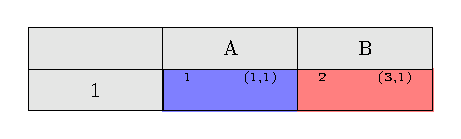
\includegraphics[scale=\figscale]{tikz/2dims1}}\hspace{2em}
    % \subfloat[]{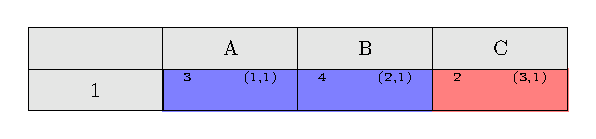
\includegraphics[scale=\figscale]{tikz/2dims2}}\\
    % \noindent 
    % \subfloat[]{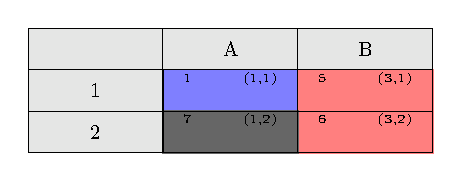
\includegraphics[scale=\figscale]{tikz/2dims3}}\hspace{2em} 
    % \subfloat[]{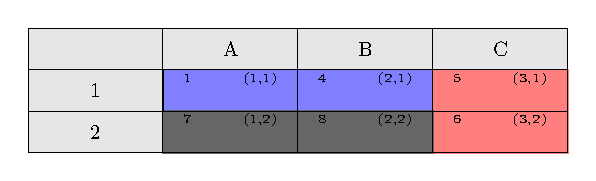
\includegraphics[scale=\figscale]{tikz/2dims4}}
% \caption{For Variants of a Variational Spreadsheet}
% \label{fig:fourvar}
% \end{figure*}


\section{Partial Tag Selection and Goal-Directed Selection}
\newcommand{\ptsel}[2][s]{\OB{{\lfloor#2\rfloor}^p_{#1}}}
\newcommand{\compatibleSym}{\OB{\sim}}
\newcommand{\compatible}[2]{\OB{#1\compatibleSym#2}}
\newcommand{\updateText}{\textit{update}}
\newcommand{\update}[2]{\updateText(#1, #2)}

Variation semantics works with complete decisions, which is applicable
when users could make decisions for all dimensions. In practice, 
users might not know all decisions in advance. They might make decisions
for some dimensions, observe the outcome, and then either undo or reiterate the process.
We introduce the notion of \emph{partial tag selection} to support users
in making partial decision. Partial tag selection takes a variational
spreadsheet and a decision as input and returns another variational spreadsheet. 
When the input is a complete decision, partial tag selection returns a variant.
For instance, when applying the incomplete decision \dset{\mapname{\htdim.Close}}
on the spreadsheet in Figure~\ref{fig:mspending}, we obtain a spreadsheet
with \mapname{\lpdim} as the only dimension and the costs of housing and transportation become non-variational.  
 
Formally, the partially tag selection operation $\ptsel[]{} : \VSheet \times 2^{\tg} \rightarrow \VSheet$ is defined as
\[
\ptsel[ts]{\vsheet} = \{\update{c}{ts}\ |\ c \leftarrow \vsheet, \compatible{\tagsCell{c}}{ts} \}
\]

\noindent
The \updateText~operation removes all tags in \OB{ts} from cell \OB{c}'s tags.
If $\tagsCell{c} \subseteq ts$, \OB{c}'s tags becomes empty and the cell becomes
non-variational. The \compatibleSym~relation returns true if two sets of tags do not have
conflicts in decisions, that is, for every shared dimension,
corresponding tags must be the same. 
For instance, \compatible{\dset{D_1.t_1, D_2.t_2}}{\dset{D_1.t_1}} holds while \compatible{\dset{D_1.t_1, D_2.t_2}}{\dset{D_1.{t_1'}, D_2.t_2}} does not.

\[
\compatible{ts_1}{ts_2} = \forall D, D.{t_1} \in ts_1 \wedge D.{t_2} \in ts_2 \rightarrow t_1 = t_2
\]

Goal-directed selection is defined as partial tag selection on variational spreadsheets. Users
begin by inspecting all possible values of a cell. In Figure~\ref{fig:selection},
the cell being inspected is \prog{B8} and has four possible values, each
corresponding to a partial decision (In this example specifically, the partial decisions happen to be the complete decisions). The alternative \OB{1450} corresponds
to the decision \mapname{\{\htdim.Close, \lpdim.500\}}, which could be applied to
 the spreadsheet to obtain a single variant.

We simplify our discussion by looking four variants of a simpler spreadsheet in Table~\ref{tbl:costcalc}...


\begin{table*}
\centering
  \begin{tabular}{|>{\centering\arraybackslash}m{2em}|>{\centering\arraybackslash}m{25em} >{\centering\arraybackslash}m{25em}|}
    \hline
    & $D_1$ & $D_2$ \\ \hline
    $D'_1$ & 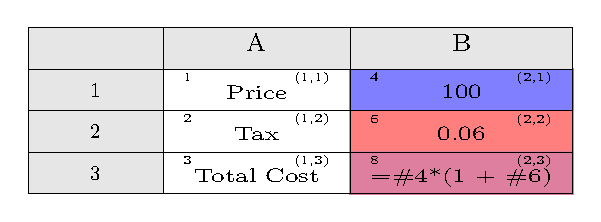
\includegraphics[scale=\figscale]{tikz/costs1}
      & 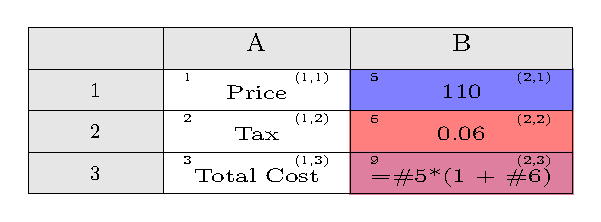
\includegraphics[scale=\figscale]{tikz/costs2} \\
      $D'_2$ & 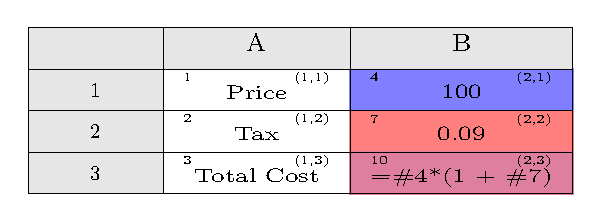
\includegraphics[scale=\figscale]{tikz/costs3} %\fixedlabel{fig:2dims3}{tikz/2dims3} 
      & 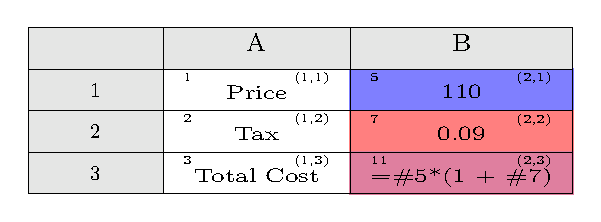
\includegraphics[scale=\figscale]{tikz/costs4} \\ \hline
  \end{tabular}
  \caption{Four Variants of the Receipt Spreadsheet}\label{tbl:costcalc}
\end{table*}



\NOTE{TODO: (0) Provide a simpler example to talk about goal directed selection and syntactic sugar, (1) Talk about syntactic sugar (address referencing) here to enable \gds, (2) Describe \gds~ in more details, (3) Syntactic revisit: how to show all variants of a cell at a certain address?}

\section{Language Properties}
\label{sec:langprops}

\begin{theorem}
If \compatible{ts_1}{ts_2} and $ts_1 \cap ts_2 = \emptyset$,
\[
\tsel[ts_1 \cup ts_2]{\vsheet} = \ptsel[ts_2]{\ptsel[ts_1]{\vsheet}} = \ptsel[ts_1]{\ptsel[ts_2]{\vsheet}}
\]
\end{theorem}

\begin{proof}
...
\end{proof}



\NOTE{TODO: Add three more theorems: (1) C-S equivalent (choice expansion), (2) Reduction of tags, (3) Dimension dependency theorem}

% \NOTE{Some laws are: (1) Orders does not matter when performing tag selection.
% (2) What about the composition of two variational spreadsheets?
% (3) What does the addressing scheme affect the representation?
% }

\section{Conclusion and Future Work}
\label{sec:concl}
TBD

\bibliographystyle{abbrv}
\bibliography{change}

\end{document} 